\documentclass{article}
\usepackage[utf8]{inputenc}
\usepackage[margin=1.2in]{geometry}
\usepackage[T1]{fontenc}                
\usepackage[utf8]{inputenc}             
\usepackage[english,portuguese]{babel}
\usepackage{hyperref}

\usepackage{tikz}
\usetikzlibrary{positioning}

\usepackage{natbib}
\usepackage{graphicx}
\usepackage{amsmath}
\usepackage{listings}
\usepackage{xcolor}


\definecolor{codegreen}{rgb}{0,0.6,0}
\definecolor{codegray}{rgb}{0.5,0.5,0.5}
\definecolor{codepurple}{rgb}{0.58,0,0.82}
\definecolor{backcolour}{rgb}{0.95,0.95,0.92}
\definecolor{deepblue}{rgb}{0,0,0.5}
\definecolor{deepred}{rgb}{0.6,0,0}
\definecolor{deepgreen}{rgb}{0,0.5,0}

\lstdefinestyle{mystyle}{
    backgroundcolor=\color{white},   
    commentstyle=\color{codegreen},
    keywordstyle=\color{deepblue},
    numberstyle=\tiny\color{codegray},
    stringstyle=\color{deepgreen},
    emph={Agent,__init__,act,self,union,exists, scope},
    emphstyle=\color{deepred},
    basicstyle=\ttfamily\footnotesize,
    breakatwhitespace=false,         
    breaklines=true,                 
    captionpos=b,                    
    keepspaces=true,                 
    numbers=left,                    
    numbersep=5pt,                  
    showspaces=false,                
    showstringspaces=false,
    showtabs=false,                  
    tabsize=3
}

\lstset{style=mystyle}



\title{Árvores de Descisão e Redes Neurais Artificiais}
\author{Prof. Rodrigo Pedrosa}

\usepackage{natbib}
\usepackage{graphicx}
\usepackage{amsmath}
\PassOptionsToPackage{hyphens}{url}\usepackage{hyperref}

\begin{document}

\maketitle

\vspace{-1.2cm}

\section{Árvores de decisão}

    \begin{enumerate}

    \item O que é uma árvore de decisão e como ela é usada na aprendizagem de máquina?

    \item Qual é a diferença entre os algoritmos de construção de árvore de decisão para classificação e para regressão?

    \item O que podemos fazer para evitar o \textit{overfitting} em árvores de decisão?

    \item Considere um conjunto de dados com 100 exemplos, dos quais 60 pertencem à classe A e 40 pertencem à classe B. Calcule o índice de Gini desse conjunto de dados.

    \item Em um conjunto de dados com 80 exemplos, dos quais 45 pertencem à classe X e 35 pertencem à classe Y. Calcule o índice de Gini desse conjunto de dados.

    \item Suponha que um conjunto de dados seja dividido em dois subconjuntos, onde o subconjunto A contém 30 exemplos, dos quais 20 pertencem à classe P e 10 pertencem à classe Q, e o subconjunto B contém 70 exemplos, dos quais 40 pertencem à classe P e 30 pertencem à classe Q. Calcule o ganho de Gini para essa divisão com base no índice de Gini inicial do conjunto de dados.

   \item Considere um conjunto de dados com duas características, "Altura" (com valores "Alto" e "Baixo") e "Idade" (com valores "Jovem" e "Adulto"), e uma classe "Classe" (com valores "A" e "B"). 
   
   Considere a seguinte tabela de dados:

    \begin{center}
    \begin{tabular}{ |c|c|c| }
    \hline
    Altura & Idade & Classe \\
    \hline
    Alto & Jovem & A \\
    Alto & Adulto & A \\
    Baixo & Jovem & B \\
    Baixo & Adulto & B \\
    Alto & Jovem & B \\
    Baixo & Adulto & A \\
    \hline
    \end{tabular}
    \end{center}
   
   Construa uma árvore de decisão para classificar os exemplos com base nessas características, usando o critério de Gini.

   \item Dado um conjunto de dados com 100 exemplos, onde 70 pertencem à classe X e 30 pertencem à classe Y, avalie duas divisões possíveis com base no índice de Gini, e determine qual delas é mais preferível em termos de impureza.

   \item Considere a seguinte base de dados:
    
   \begin{figure}[!ht]
        \centering
        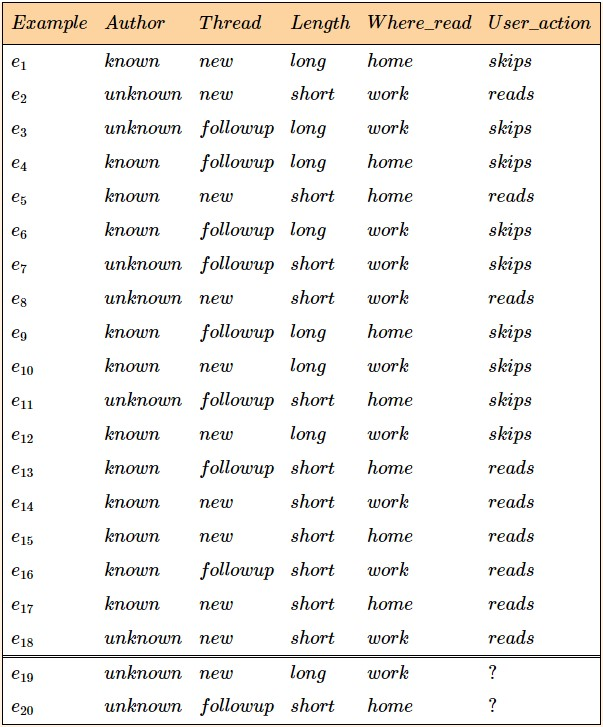
\includegraphics[width=0.55\textwidth]{abc.jpg}
   \end{figure}


       \begin{enumerate}
       
       \item Apresente uma árvore de decisão para a classificação das \textit{User-actions} e calcule o grau de impureza ($I_G$) médio do nó raiz da sua árvore. (Obs: $I_G(p) = 1 - \sum_{i=1}^{J}p_i^2$)
           
       \item De acordo com a árvore apresentada, qual a classificação dos exemplos $e_{19}$ e $e_{20}$?  
       
       \end{enumerate}

    \end{enumerate}
    
    \section{Redes Neurais Artificiais}

    \begin{enumerate}
        \item  Considere a rede neural abaixo:
    
    \begin{figure}[!ht]
        \centering
        \begin{tikzpicture}[%
            neuron/.style={circle, draw, thick, minimum size=1cm},
            arrow/.style={->,>=stealth,thick}
        ]
        
        % Input neurons
        \node[neuron] (input1) at (0,0) {$x_1$};
        %\node[neuron] (input2) [below=of input1] {$x_2$};
        
        % Hidden layer neurons
        \node[neuron] (hidden1) [right=2cm of input1] {};
        \node[neuron] (hidden2) [below=of hidden1] {};
        
        % Output neuron
        \node[neuron] (output) [right=2cm of hidden1, yshift=-1.25cm] {};
        
        % Connect input layer to hidden layer
        \draw[arrow] (input1) -- (hidden1) node[midway, above] {$w_{21}$};
        \draw[arrow] (input1) -- (hidden2) node[near start, above] {$w_{22}$};
        %\draw[arrow] (input2) -- (hidden1) node[near start, below] {$w_{12}$};
        %\draw[arrow] (input2) -- (hidden2) node[midway, below] {$w_{22}$};
        
        % Connect hidden layer to output layer
        \draw[arrow] (hidden1) -- (output) node[midway, above] {$w_{31}$};
        \draw[arrow] (hidden2) -- (output) node[midway, below] {$w_{32}$};
        
        \end{tikzpicture}
    \end{figure}

    Esta rede não possui termos de viés (bias) e tem como funções de ativação a função ReLU (Rectified Linear Unit) que pode ser definida como:

    \begin{equation}
        \text{ReLU}(x) = \max(0, x)
    \end{equation}

    A derivada da ReLU é definida como:

    \begin{equation}
            \frac{d}{dx}(\text{ReLU}(x)) =
            \begin{cases}
            1 & \text{if } x > 0 \\
            0 & \text{if } x \leq 0
            \end{cases}            
    \end{equation}

    Obtenha o gradiente do erro quadrado em relação aos pesos da rede. Todos os passos da derivação da gradiente devem ser apresentados.

    \item  Considere a rede neural abaixo:
    
    \begin{figure}[!ht]
        \centering
        \begin{tikzpicture}[%
            neuron/.style={circle, draw, thick, minimum size=1cm},
            arrow/.style={->,>=stealth,thick}
        ]
        
        % Input neurons
        \node[neuron] (input1) at (0,0) {$x_1$};
        \node[neuron] (input2) [below=of input1] {$x_2$};
        
        % Hidden layer neurons
        \node[neuron] (hidden1) [right=2cm of input1] {};
        \node[neuron] (hidden2) [right=2cm of input2] {};
        
        % Output neuron
        \node[neuron] (output) [right=2cm of hidden1, yshift=-1.25cm] {};
        
        % Connect input layer to hidden layer
        \draw[arrow] (input1) -- (hidden1) node[midway, above] {$w_{11}$};
        \draw[arrow] (input1) -- (hidden2) node[near start, above] {$w_{21}$};
        \draw[arrow] (input2) -- (hidden1) node[near start, below] {$w_{12}$};
        \draw[arrow] (input2) -- (hidden2) node[midway, below] {$w_{22}$};
        
        % Connect hidden layer to output layer
        \draw[arrow] (hidden1) -- (output) node[midway, above] {$w_{31}$};
        \draw[arrow] (hidden2) -- (output) node[midway, below] {$w_{32}$};
        
        \end{tikzpicture}
    \end{figure}

    $w_{11}$ = $w_{21}$ = $w_{12}$ = $w_{22}$ = $w_{31}$ = $w_{32}$ = 1

    Esta rede tem como funções de ativação a função ReLU (Rectified Linear Unit) que pode ser definida como:

    \begin{equation}
        \text{ReLU}(x) = \max(0, x)
    \end{equation}

    A derivada da ReLU é definida como:

    \begin{equation}
            \frac{d}{dx}(\text{ReLU}(x)) =
            \begin{cases}
            1 & \text{if } x > 0 \\
            0 & \text{if } x \leq 0
            \end{cases}            
    \end{equation}


    \begin{enumerate}
        \item Calcule o gradiente do erro quadrado em relação à $w_{32}$ quando $\mathbf{x} = [2,1]$ e $y = 20$.
        \item Calcule o gradiente do erro quadrado em relação à $w_{22}$ quando $\mathbf{x} = [2,1]$ e $y = 20$. 
        \item Como $w_{32}$ e $w_{22}$ devem ser alterados de forma a diminuir o erro?   
    \end{enumerate}
    
    \item Quais são as funções de ativação mais comuns usadas nas redes neurais artificiais e como elas afetam o processo de treinamento?

    \item Como o \textit{overfitting} pode ser evitado em redes neurais artificiais?
    
  \end{enumerate}

  \section{Overfitting, Underfitting e Avaliação de Modelos}

\subsection{Conceitos fundamentais}
\begin{enumerate}
  \item Defina \textit{overfitting} e \textit{underfitting}. Dê um exemplo de situação que tipicamente leva a cada um deles.
  \item Explique o \textit{trade-off} viés–variância. Como esse \textit{trade-off} se manifesta quando aumentamos a complexidade do modelo?
  \item Diferencie erro de aproximação (viés) e erro de estimação (variância). Por que ambos importam?
  \item Em que sentido as regularizações L1 e L2 ajudam a mitigar overfitting? Compare seus efeitos esperados sobre os coeficientes.
  \item O que é \textit{capacidade do modelo}? Relacione capacidade, número de parâmetros e risco de overfitting.
  \item Explique \textit{early stopping}. Por que ele pode ser visto como uma forma de regularização?
\end{enumerate}

\subsection{Diagnóstico e detecção}
\begin{enumerate}
  \setcounter{enumi}{6}
  \item Descreva como curvas de aprendizado (\textit{learning curves}) podem distinguir overfitting de underfitting. Que padrões você esperaria ver?
  \item Você observa alta acurácia em treino e baixa em teste. Quais hipóteses explicam esse comportamento e como investigá-las?
  \item Em um problema desbalanceado, por que acurácia pode mascarar overfitting? Sugira métricas alternativas.
  \item O que é \textit{data leakage}? Dê dois exemplos comuns de vazamento e como evitá-los.
  \item Qual o papel de um conjunto de validação separado na detecção de overfitting durante ajuste de hiperparâmetros?
\end{enumerate}

\subsection{Particionamento e validação}
\begin{enumerate}
  \setcounter{enumi}{11}
  \item Diferencie conjunto de treino, validação e teste em termos de propósito. O que ocorre quando usamos o teste para escolher hiperparâmetros?
  \item Explique \textit{validação cruzada} k-fold. Quais são suas vantagens em relação a um único \textit{holdout}?
  \item Quando a validação cruzada \textit{estratificada} é necessária? O que ela preserva e por quê?
  \item Por que a \textit{nested cross-validation} (CV aninhada) é recomendada para comparação justa de modelos? Descreva a estrutura externa e interna.
  \item Em séries temporais, por que k-fold aleatório é inadequado? Descreva um esquema de validação temporal apropriado.
  \item Em quais situações o \textit{leave-one-out} CV (LOOCV) é vantajoso e quando pode ser problemático?
  \item Como você escolheria $k$ no k-fold? Quais impactos de $k$ muito pequeno ou muito grande sobre viés/variância da avaliação?
\end{enumerate}

\subsection{Seleção de modelos e métricas}
\begin{enumerate}
  \setcounter{enumi}{18}
  \item Diferencie \textit{seleção de modelo} de \textit{avaliação final}. Por que não devemos reportar no artigo o melhor resultado observado durante a busca de hiperparâmetros sem correção?
  \item Como escolher métricas quando os custos de erro são assimétricos? Dê exemplos de métricas apropriadas para classificação com custos diferenciados e para regressão com \textit{outliers}.
  \item Você treinou um modelo com ajuste de hiperparâmetros via CV e agora quer relatar o desempenho final. Qual procedimento correto para estimar o desempenho fora da amostra?
\end{enumerate}


  \section{Questões Práticas [opcional]}

    \begin{enumerate}
        \item Reproduza o tutorial disponível em \url{https://www.analyticsvidhya.com/blog/2021/06/end-to-end-machine-learning-use-case-for-beginners/} com os dados \url{https://www.kaggle.com/datasets/mrigaankjaswal/student-performance-in-mathematics-and-portuguese}
        \item Substitua o modelo do tutorial por uma Árvore de Decisão e faça uma análise comparativa quantitativa e qualitativa entre o modelo de Regressão Linear e a Árvore de decisão.
    \end{enumerate}


%\bibliographystyle{plain}
%\bibliography{references}

\end{document}
